\documentclass[10pt,journal,compsoc]{IEEEtran}

\pdfminorversion=7

\usepackage{amsmath,amsfonts}
\usepackage{algorithmic}
\usepackage{array}
\usepackage[caption=false,font=normalsize,labelfont=sf,textfont=sf]{subfig}
\usepackage{textcomp}
\usepackage{stfloats}
\usepackage{url}
\usepackage{verbatim}
\usepackage{graphicx}
\usepackage{booktabs}
\usepackage{enumerate}
\usepackage{listings}
\usepackage{hyperref}
\usepackage{xspace}
\usepackage{balance}
\usepackage[most]{tcolorbox}
\usepackage{awesomebox}
\usepackage{multirow}
\usepackage{blindtext}

\usepackage{mdframed}
\usepackage[colorinlistoftodos]{todonotes}

\hyphenation{op-tical net-works semi-conduc-tor IEEE-Xplore}
\def\BibTeX{{\rm B\kern-.05em{\sc i\kern-.025em b}\kern-.08em
    T\kern-.1667em\lower.7ex\hbox{E}\kern-.15emX}}

%.1667


% Custom colors
\definecolor{keywords}{rgb}{0.5,0,0.35}
\definecolor{comments}{RGB}{0,0,113}
\definecolor{red}{RGB}{160,0,0}
\definecolor{green}{RGB}{0,150,0}
 
\lstset{language=Python, 
        basicstyle=\ttfamily\small, 
        keywordstyle=\color{keywords}\bfseries,
        commentstyle=\color{comments},
        stringstyle=\color{red},
        showstringspaces=false,
        %identifierstyle=\color{red},
       }
       
\newmdtheoremenv [
 outerlinewidth = 1 ,
 roundcorner = 1pt,
 leftmargin = 1,
 rightmargin = 1,
 backgroundcolor = gray!20,
 outerlinecolor = blue!70!black,
 %innertopmargin = \topskip, 
 %splittopskip = \topskip ,
 ntheorem = false,
] {finding}{Finding}

% Pictures
\usepackage{graphicx}       



\newtcbtheorem{obs}{Finding}{%
        theorem name,%
        colback=gray!5,%
        colframe=gray!35!black,%
        fonttitle=\bfseries,title after break={Lemma  -- \raggedleft Continued}%
    }{lem}


% \newcommand{\pw}{Chapter~\ref{chap:large-study}}    
% \newcommand{\pw}{\ref{}}    
\newcommand{\pw}{in Chapter~5}

% \newcommand{\chap}{section}
\newcommand{\chap}{chapter}

\newcommand{\tb}[2]{\tipbox{{\bf Finding #1}. #2}}

\newcommand{\droidxp}{DroidXP\xspace}
\newcommand{\droidxpflow}{DroidXPflow\xspace}
\newcommand{\review}[1]{\textcolor{black}{#1}}
\newcommand{\alert}[1]{\textcolor{red}{#1}}
\newcommand\kn[1]{\textcolor{red}{KN: #1}}
\newcommand\fh[1]{\textcolor{green}{FH: #1}}
\newcommand\rb[1]{(\textcolor{red}{RB: #1})}

\newcommand{\highlight}[1]{{\color{red}}#1}

\newcommand\raw[1]{\textcolor{red}{#1}\xspace}

\newcommand{\mas}{MAS approach\xspace}

\newcommand{\net}{Network Traffic Analysis\xspace}

\newcommand{\ml}{ML process\xspace}

\newcommand{\fm}[1]{\emph{#1}\xspace}

\newcommand{\gps}{\fm{gappusin}}  % the gappusin family.
\newcommand{\rmb}{\fm{revmob}}
\newcommand{\dwg}{\fm{dowgin}}

\newcommand{\tjk}{\fm{torjok}}

\newcommand{\sscore}{Similarity Score\xspace}

\newcommand{\rqa}{How much gain we obtain on the accuracy of Android malware classification when considering network flow data and ML?}

\newcommand{\rqb}{Which algorithms are effective to be used for training models base on network traffic data and ML for malware identification?}

\newcommand{\rqc}{Which  malware families (e.g., \fm{gappusin}, \fm{kuguo}, \fm{dowgin}) the Flow Analysis has the best performance, and in which families the proposal is not so efficient?}

\newcommand{\rqe}{How much gain we obtain on the performance of the \mas for malware classification when considering its extensions?}


\newcommand{\repack}{RePack\xspace}
\newcommand{\amc}{AndroMalPack\xspace}

\newcommand{\appsSmall}{102\xspace}
\newcommand{\apps}{\textcolor{black}{4,076}\xspace}
\newcommand{\napps}{\textcolor{blue}{726}\xspace}

\newcommand{\sds}{\texttt{SmallDS}\xspace}
\newcommand{\cds}{\texttt{LargeDS}\xspace}
\newcommand{\fds}{\texttt{FlowDS}\xspace}
\newcommand{\nds}{\texttt{DS3}\xspace}
\newcommand{\avt}{\texttt{avclass2} tool\xspace}
\newcommand{\vt}{\texttt{VirusTotal}\xspace}
\newcommand{\se}{security engine\xspace}
\newcommand{\ses}{security engines\xspace}


\newcommand{\fone}{F1-score\xspace}
\newcommand{\fscoreSmall}{0.89\xspace}
\newcommand{\fscoreNew}{0.85\xspace}

\newcommand{\nfscoreSmall}{0.85\xspace}
\newcommand{\nfscoreSmallC}{0.87\xspace}

\newcommand{\fscore}{\textcolor{black}{0.54}\xspace}
\newcommand{\fscoreC}{\textcolor{blue}{0.49}\xspace}

\newcommand{\malwares}{\textcolor{black}{2,895}\xspace}
\newcommand{\malwaresP}{\textcolor{black}{71.02}}
\newcommand{\malwaresN}{\textcolor{blue}{87.98}}
\newcommand{\appsGps}{\textcolor{black}{1,337}\xspace}
\newcommand{\appsGpsFN}{\textcolor{black}{1,170}\xspace}
\newcommand{\fhc}{FHC-Study\xspace}
\newcommand{\blls}{BLL-Study\xspace}


\begin{document}

\title{Using Network Flow Data and Machine Learning as Support for Mining Android Sandbox}


\author{Francisco Costa,
        Roberto Valera, 
        Rodrigo~Bonif\'{a}cio,
        Eduardo Gomes, 
        Jo\~{a}o Gondim
\IEEEcompsocitemizethanks{
\IEEEcompsocthanksitem F. Costa, R. Valera, R. Bonif\'{a}cio, E. Gomes and J. Gondim are with the 
Computer Science Department, University of Bras\'{i}lia, Bras\'{i}lia, Brazil.
E-mail: \{francisco.costa\}@aluno.unb.br and \{roberto.luis,rbonifacio,edumonteiro,gondim\}@unb.br.

}
}



\IEEEtitleabstractindextext{
\begin{abstract}
As mobile technologies become part of modern society, Android's dominance in the global smartphone market has made it a prime target for cyberattacks. The Android platform faces a growing threat from malware, particularly repackaged apps that embed malicious code to exploit user data. While sandbox-based approaches, such as Mining Android Sandbox (MAS), have been effective in detecting repackaged malware by analyzing sensitive API interactions, they often fall short in identifying more complex threats. This paper introduces a complementary approach that integrates network flow analysis with \mas to improve malware detection. By analyzing the network traffic generated by Android applications, alongside behavioral data from \mas, this method uncovers malicious activities that may remain hidden within the app’s behavior. Using machine learning on network traffic data collected via TcpDump, combined with \mas insights, our method improves the accuracy of malware detection. Results demonstrate that this combined approach significantly improves the identification of malware, offering a more comprehensive solution for securing Android applications against evolving threats.
\end{abstract}
}





\maketitle
\begin{IEEEkeywords}
Android Malware Detection, Dynamic Analysis, Network Traffic Analysis, Smartphone, Mining Android Sandboxes.
\end{IEEEkeywords}

\section{Introduction}\label{sec:introduction}


Android is a robust Linux-based operating system widely used in mobile technology. It has more than $2.5$ million Android applications~\footnote{In this paper, the terms Android Applications, Android Apps, and Apps will be used interchangeably to refer to software applications for the Android platform.} (apps) available in the official Google Play Store until June 2023~\cite{Statista}. As its popularity rises, so does the risk of potential attacks, making Android-based devices prime targets for malicious apps (malware). In general, the main aim of malware is to gain unauthorized access to and exploit sensitive resources on a device~\cite{DBLP:conf/ccs/FeltFCHW11,DBLP:journals/eswa/SurendranTE20}.
This can lead to various risks, including disrupted device functionality, battery drain, information leakage, and other threats~\cite{DBLP:conf/ccs/FeltFCHW11,DBLP:conf/sp/ZhouJ12}.

A prevalent form of Android malware involves repackaging legitimate apps~\cite{DBLP:conf/wcre/BaoLL18, le2018towards}. These malicious variants can insert or modify the original apps with harmful code and release them on (un)official third-party markets~\cite{DBLP:journals/tdsc/TianYRTP20}. Researchers~\cite{DBLP:journals/tdsc/TianYRTP20,DBLP:conf/sp/ZhouJ12,DBLP:journals/compsec/MerloRSV21} show that the $86\%$ of Android malicious apps are repackaged, highlighting theprevalence of this approach to inject malicious behavior. To counter this, several general-purpose Android malware detection techniques have been developed. For example, the Mining Android Sandbox (hereafter \mas) for malware detection, adapted from~\cite{DBLP:conf/icse/JamrozikSZ16}, relies on the calls to sensitive APIs to check whether a repackaged version of an app is malicious or not~\cite{DBLP:conf/wcre/BaoLL18,DBLP:jourals/jjc/Handrick22}. The original \mas leverages static and dynamic analysis on Android app to protect sensitive resources at a fine-grained level by limiting access to sensitive APIs.

Focused on app behavior abstraction, the \mas has proven effective in detecting repackaged malware, as demonstrated in previous work~\cite{DBLP:conf/wcre/BaoLL18}, which classified as malware 77 out of 102 app pairs (original and repackaged versions of an app)~\footnote{Hereafter, when we use the term app pair(s), we refer to original and repackaged versions of an Android application}. However, the study by Bao et al.~\cite{DBLP:conf/wcre/BaoLL18} (\blls), evaluated the technique using a dataset comprising only 102 app pairs, with a limited number of malware families. Using the same dataset from \blls, Costa et al.~\cite{DBLP:jourals/jjc/Handrick22}, present an in-depth analysis of \mas highlighting the contributions of the static and dynamic analysis components to malware detection, bringing evidence that both techniques complement each other. 

Further exploration of the \mas was also discussed \pw, which revealed the need for additional studies using datasets larger than used in the \blls. The research presents an empirical evaluation of the \mas using a larger dataset (hereafter referred to as \cds), which contains $4,076$ app pairs and $116$ malware families. That previous study also showed evidence that, when applied to the \cds, the accuracy of the \mas drops significantly, with an \fone of $0.54$. This suggests that the effectiveness of the \mas in detecting and preventing malicious behaviors may not be generalizable to larger datasets. 

Motivated by the negative results reported in our previous research, in this \chap, we (a) leverage our
\droidxp infrastrucutre~\cite{DBLP:conf/scam/CostaMCMVBC20} to collect the network traffic of the apps (while they execute using a
test generation tool like DroidBot~\cite{DBLP:conf/icse/LiYGC17}) and (b) explore machine learning (ML) algorithms to classify
the repackaged version of the apps as malware / non-malware using network traffic data. The results
of the experiments that we present here show that combining the \mas with the ML technique we
detail in this paper leads to an accuracy (\fone) of 0.89. This improvement is particularly significant for malware
families that previously exhibited high false negative rates in our earlier study. Altogether, the main
contributions of this paper are:

\begin{itemize}
  \item {\bf \droidxpflow:} a novel dynamic analysis approach for Android malware detection that relies on network traffic data
  collected using the first phase of the \mas and ML algorithms.

  \item {\bf An empirical study:} that brings evidence that \droidxpflow outpeforms the \mas. In particular, \droidxpflow
  is able to correctly classify the malware families (such as Gappusin) the original version of the
  \mas approach was not. 
\end{itemize}

The main implication of this research is that we shed light to
a possible limitation of the \mas in general. We argue that
robust sandboxes should consider not only the calls to
sensitive APIs, but also monitor network traffic data and the
access to native resources to detect possible malicious
behavior of Android apps.

% \textbf{Our contribution:} Altogether, the main contribution of this paper is two-fold: first, we propose \droidxpflow,
% a framework designed to detect malicious apps based on dynamic analysis of network traffic and ML algorithms.
% To achieve this, the framework collects traffic generated by both original and repackaged versions of the apps using an extension
% of \droidxp~\cite{DBLP:conf/scam/CostaMCMVBC20}. In addition to gathering data related to calls to sensitive APIs, the \droidxp extension also captures network traffic data from the apps using the TcpDump tool. Feature engineering is then applied to extract and select relevant features for training, and characterizing network flows as either benign or malicious using supervised ML algorithms. Second, we generate a labeled and balanced dataset called \fds of benign and malicious flows using the CICFlowMeter~\cite{DBLP:conf/icissp/LashkariDMG17} software. This dataset contains more than $3,000$ network traffic features, extracted from $2,958$ benign apps and $2,886$ malicious apps spanning 116 malware families.\newline\newline

% \textbf{Organization.} The rest of the paper is organized as follows: Section~\ref{sec:background} highlights the background and related work. Section~\ref{sec:Methodology} discuss the studies setting in details. The results of your approach are discussion in Section~\ref{sec:results}. After present implications and limitations at Section~\ref{sec:discussion}, we close with conclusion at Section~\ref{sec:conclusions}.



\section{Background and Related Work}\label{sec:background}

Extensive research has focused on pre-installation Android malware detection through static and dynamic analysis. Dynamic approaches, like TaintDroid~\cite{DBLP:conf/osdi/EnckGCCJMS10}, DroidRanger~\cite{Zhou2012HeyYG}, and DroidScope~\cite{LKYanDroidscope}, monitor app behavior in real-time, offering high accuracy but significant performance overhead, limiting their practical use on mobile devices. In contrast, static methods such as Kirin~\cite{Enck2009}, Stowaway~\cite{DBLP:conf/ccs/FeltCHSW11}, and RiskRanker~\cite{GraceRiskranker2012} are efficient and scalable but heavily rely on manually defined patterns, hindering their effectiveness against novel malware. Additionally, these methods often lack transparency, making it difficult to understand their decision-making processes. The lack of understanding about Mining Android Sandbox also appears in the work of Francisco et al. (hereafter \fhc), which presents an empirical study that explores the performance of \mas when using a large dataset of pair of apps for identifying malicious behavior.

\subsection{Mining Android Sandbox}

A sandbox is a controlled environment that isolates applications from the host system, preventing them from accessing or modifying files, networks, or other device data ~\cite{DBLP:journals/peerj-cs/MaassSCS16}. This isolation allows for safe testing and execution of potentially malicious code without compromising the device's integrity~\cite{DBLP:conf/esorics/BordoniCS17}. Such a need arises in various scenarios, including when dealing with untrusted user input, analyzing malware, or mitigating risks in compromised systems~\cite{DBLP:journals/peerj-cs/MaassSCS16}. A sandbox must protect the host machine and operating system from any harm caused by third-party software. To achieve this, it should provide the minimum necessary resources for program execution, ensuring that the program does not impact external resources.

The \mas ~\cite{DBLP:conf/icse/JamrozikSZ16} employs test generation tools to examine an Android app's dynamic behavior and identify essential sensitive resources. By restricting access to these specific APIs, the sandbox safeguards app execution. The process involves two stages. In the exploratory phase, a benign app version is executed using test generation tools, recording the utilized sensitive APIs. Subsequently, during the execution phase, the sandbox limits the app's access to only the previously identified sensitive APIs, preventing malicious apps from accessing any unauthorized sensitive resources.

Beyond its ability to generate Android sandboxes, the MAS approach is also effective in identifying malicious behavior in repackaged Android apps~\cite{DBLP:conf/wcre/BaoLL18}. The effectiveness of this approach is measured by its accuracy in correctly flagging malicious activities within repackaged versions of applications. In ~\cite{DBLP:jourals/jjc/Handrick22} the authors explore the use of static and dynamic analysis to improve the performance of the \mas. They propose a new approach based on taint analysis for malware identification demonstrating that when combining taint analysis with \mas, the percentage of malware identification is increased. Despite this results, both \mas and taint analysis present limitations that can be overcome using other approaches like, machine learning.

\subsection{Network Traffic Analysis}

Due to the previously mentioned limitations of static and dynamic analyses, researchers begin to analyze and identify malicious apps using network traffic. For example, signature-based detection methods assess malware by comparing it to known malware patterns. Griffin et al.~\cite{Griffin2009}  used 48-byte code sequences as signatures. Researchers have also explored automatically generating network signatures~\cite{PolygraphNewsome2005, Singh2004, Yegneswaran2005}, often focusing on worm identification. Perdisci et al. ~\cite{Perdisci2010} generated network signatures for mobile malware based on HTTP traffic, analyzing similarities and clustering malicious patterns. While effective against known threats, signature-based methods struggle to detect novel attacks due to their reliance on predefined patterns.

Some studies utilize text analysis for malware detection based on Packet/Flow textual features. Nan et al.~\cite{yuhong:usenix-2015} introduced UIPicker, a framework that uses NLP, machine learning, and program analysis to identify personal user information on a large scale. N-grams, a technique from NLP, have been applied to network protocol identification~\cite{YunWang2016}. Recon et al. ~\cite{ren:mobisys-2016} recently proposed a method to detect and prevent personal information leaks in mobile network traffic by analyzing key-value pairs. Some authors has also used Packet/Flow features statistically. Arora et al.~\cite{arora:ngmast-2014} compared malware traffic to benign network traffic, identifying deviations in network behavior using statistical features like average packet size, flow duration, and byte ratios. AppScanner~\cite{taylor:eurosp-2016} is a framework that uses statistical features of encrypted network traffic to automatically fingerprint and identify Android apps. Conti et al.~\cite{Conti2016} [19] analyzed encrypted Android traffic to identify user actions based on statistical features. However, statistical feature-based methods can have a high error rate due to their coarse-grained traffic characterization.

\subsection{Machine Learning Approach}

Machine learning approach has been used in network traffic-based malware detection methods. Depending on the type of machine learning model used, these methods can be divided into two categories: (1) shallow learning techniques and (2) deep learning techniques. Shallow learning usually relies on handcrafted features based upon the target problem. These techniques include classic machine learning methods such as decision tree, random forest, KNN, and SVM. In contrast, deep learning methods are able to derive their own features directly from data by different hidden neural network layers.

 Shallow techniques traditionally are used in malware detection methods as a classification problem. Researchers~\cite{RIBEIRO2020} have developed a host-based application to monitor device resource usage (e.g., CPU, memory, battery) and detect malware with over $90$\% accuracy using statistical and machine learning methods. Chen et al.~\cite{CHEN2018346} investigated the impact of data imbalance on Android malicious flow detection, finding that it can significantly reduce accuracy. They experimented with various classifiers on imbalanced datasets, demonstrating the effectiveness of machine learning for identifying malicious mobile traffic. Another study~\cite{lashkari:pst-2017} analyzed network traffic features to distinguish malicious traffic from normal traffic and identify malware types, using common classifiers like regression, KNN, decision trees, and random forests.

 %Research on deep learning-based malware detection using traffic analysis is limited. Alzaylaee et al.~\cite{ALZAYLAEE2020101663} developed a deep learning model to detect malicious Android apps using static and dynamic features. Wang~\cite{wang:iwqos-2018} proposed a URL-based malware detection method using a multi-view neural network. This network automatically creates multiple views of URLs and assigns attention weights to focus on different features. The method demonstrated high accuracy in detecting malware from different months of a specific year.



\section{Methodology}\label{sec:Methodology}

In this section, our goal is to build an in-depth understanding of the network traffic generated by apps at the network access point, and investigate how this traffic can improve the performance of the \mas for detection of malicious apps. To achieve this goal, we investigate the following research questions:

\begin{enumerate}[(RQ1)]
\item \rqa
\item \rqb
\item \rqc
% \review{\item \rqe}
\end{enumerate}

In rest of the section, we discuss our study settings as follows. First, we present how we curated an Android repackaged apps dataset that spanned a diverse range of malware families (Section~\ref{sec:dataset}). Second, we presented how \mas collect data from sensitive APIS calls, from original and repackaged apps, and how our platform also extracted network traffic generated by these apps at the network access point (Section~\ref{sec:mas}) and (Section~\ref{sec:traffic}).  Then, we explain how we collected features from this traffic (Section~\ref{sec:extraction}). Finally, we described the procedures we used to detect malicious behaviors in repackaged apps based on machine learning and how we interpreted the results (Section~\ref{sec:learning}) and (Section~\ref{sec:understand}).

\subsection{Malware Dataset}\label{sec:dataset}


To test and evaluate our proposal, we used the same dataset built by the \fhc. The dataset (hereafter referred to as \cds) contains 4,076 real-world app pairs from three repackaged app repositories (\repack~\cite{DBLP:journals/tse/LiBK21}, \amc~\cite{rafiq2022andromalpack} and Androzoo repository~\cite{DBLP:conf/msr/AllixBKT16}), along with their respective original apps. Of these, $1,777$ are original versions, and $4,076$ are repackaged versions—multiple repackaged versions of the same original app may coexist within the \cds dataset.

To ensure that all original apps were not malware, the authors queried the \vt repository, confirming that no antivirus engines flagged them as malicious. \vt is a popular tool used by researchers and practitioners to check software assets, including Android apps, using more than 60 security engines~\cite{DBLP:journals/ese/KhanmohammadiEH19}. The authors also evaluated the repackaged versions with \vt and confirmed that $71.02$\% of the repackaged apps were malicious (2,895 out of the 4,076 repackaged apps).

The \cds contains information about malware families, the similarity between the original and repackaged app versions, and the source of the Android app store. The app store source information was obtained from the three original repackaged app repositories, while the other features were extracted using the \avt~\cite{avclass2-paper} (for malware family identification) and the SimiDroid tool~\cite{DBLP:conf/trustcom/0029BK17} (for similarity scoring). According to the \fhc, the \cds comprises 116 distinct malware families, most of them from the \gps family ($46.18$\%), and an average similarity score of $90.39$\%, with the majority of app pairs ($3,587$) having more than 75\% similarity. Regarding the Android app store source, most of the repackaged apps come from the non-official Android app store, Anzhi~\cite{anzhi}.



\subsection{\mas Data Collection Procedure}\label{sec:mas}


To collect sensitive data from all apps, the \fhc leverages the DroidXP infrastructure~\cite{DBLP:conf/scam/CostaMCMVBC20}. As demonstrated in the study, DroidXP can compare test case generation tools in terms of identifying malicious app behaviors using the \mas, making it a valuable tool for automating the following steps:


\begin{enumerate}[1.]
 \item \textbf{Instrumentation}: As a first step, the \fhc uses DroidXP to instrument all pairs of apps in the \cds. Both versions of the apps are instrumented to collect relevant information during their execution. In the background, DroidXP leverages DroidFax to gather static information about all apps (both original and repackaged versions). As noted by the authors, to improve performance across multiple executions, this phase is performed only once for each version of the apps in the \cds


\item \textbf{Execution}: DroidXP then installs the instrumented version of the apps on an Android emulator. As statistical result show that $83.8\%$ of malware are activity after restart~\cite{DBLP:conf/sp/ZhouJ12}, the author report that restart the installed app, before the effective execution. Then, they initiate a test case generation tool (DroidBot~\cite{DBLP:conf/icse/LiYGC17}) to execute both versions of the app. The authors justify the use of DroidBot by citing a previous research~\cite{DBLP:conf/wcre/BaoLL18} that reports higher accuracy in sandboxes built, using the \mas combined with DroidBot as the test case generation tool. They also report that this same research indicates DroidBot’s coverage reaches near-maximum within one minute. For this reason, each app is run for one minute, and three times, to mitigate the randomness involved in test case generation tools.

\item \textbf{Data Collection}: At the end of the execution step, the \fhc once again leverages DroidFax through DroidXP, this time to collect all relevant information, such as calls to sensitive APIs. This data is then used to analyze the performance of the \mas in detecting malicious behavior.
\end{enumerate}



The study consider that a sandbox of app identifies a malware whenever the malicious app version makes a call to a sensitive API, which was not called during the exploratory phase of your original version, as present at Figure~\ref{fig:mine}.


\begin{figure*}[h]
  \centering
  
    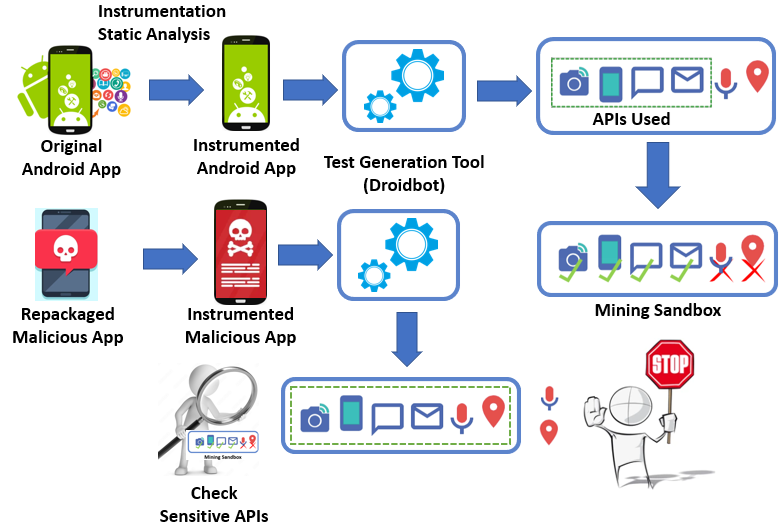
\includegraphics[width=0.55\textwidth]{image/mineSandbox.png} \\[\abovecaptionskip]
    
  \caption{Overview of \fhc for malware identification}\label{fig:mine}
\end{figure*}


\subsection{Traffic Collection Procedure}\label{sec:traffic}

To extract traffic data generated by both malicious and benign apps (4,076 app pairs), we also utilize DroidXP, which uses the TcpDump tool to collect inbound and outbound network traffic. As described in section 3.2, in the second step of our study (Execution), DroidXP also collects all packet capture (PCAP) files~\cite{DBLP:conf/iv/UhlarHR21} of all explored apps (1,182 original and 2,894 malicious). A PCAP file contains copies of trafficked packets over the network, allowing analysis of all values of payloads and packet headers~\cite{DBLP:conf/iv/UhlarHR21}. Because storing and processing PCAP files is very expensive, it is necessary to perform just a limited network segment analysis, rather than analyzing all of them. To extract the most relevant features for our study from all generated PCAP files, we utilize CICflowMeter~\cite{DBLP:conf/icissp/LashkariDMG17}, as we describe in the next section.

\subsection{Feature Extraction}\label{sec:extraction}

To extract features, we processed each traffic file (PCAP file) generated by DroidXP at explored step, creating features sets in the format of CSV files, for respective PCAP file. In the end, we combine all CSV files in just one, with total of 86 features, which we will not describe here, because of limited space. We do not considered all of them, and removed some features that were made up within at our simulated environment or do not make sense for our study like: Flow ID, Source IP, Destination IP, Source Port, Source MAC, Destination MAC, Protocol and Timestamp. In the end, we remain with 78 features.

Secondly, we filtered our CSV file by the feature "Destination Port." We used only the 15 most relevant Destination Ports, which are the ones that appear most frequently in our CSV file. (see Table~\ref{tab:port}).

\begin{table}[ht]
  \caption{THE 15 MOST RELEVANT DESTINATION PORT.}
  \centering
  \begin{small}
    \begin{tabular}{rrlrr}   \hline
 \# & Port & Description & Occurs  \\ \hline

1 &  443 &  Hypertext Transfer Protocol Secure &  1275293  \\ 
  2 &  53 & Domain Name System & 641965  \\ 
  3 &  80 & Hypertext Transfer Protocol &  38830  \\ 
  4 &  853 & DNS over TLS &  32784  \\ 
  5 &  5228 & Google Cloud Messaging &  26509  \\ 
  6 &  123 & Network Time Protocol & 9179  \\ 
  7 &  68 & Dynamic Host Configuration Protocol &  8091  \\ 
  8 &  67 & Dynamic Host Configuration Protocol &  8091  \\ 
  9 &  9999 & HyperSQL Database &  268  \\ 
  10 & 8080 & Hypertext Transfer Protocol & 221  \\ 
  11 & 6881 & BitTorrent Protocol & 173  \\ 
  12 & 5566 & Network Monitoring & 110  \\ 
  13 & 8881 & Hypertext Transfer Protocol & 110  \\ 
  14 & 9002 & Management Interfaces & 106  \\ 
  15 & 7 & Echo Protocol & 84  \\ 
   \hline

 \end{tabular}
 \end{small}
 \label{tab:port}
 \end{table}


\begin{table}[ht]
  \caption{STATISTICAL FUNCTIONS AT FEATURES.}
  \centering
  \begin{small}
    \begin{tabular}{rllrr}   \hline
 \# & Function & Description\\ \hline

1 &  min &  Minimum\\ 
  2 &  max & Maximum\\ 
  3 &  sum & Amount\\ 
  4 &  mean & Average\\ 
  5 &  std & Standard deviation \\ 
  6 &  median & Median\\ 
  7 &  count & Number of observation\\ 
  8 &  var & Variance\\ 
  9 &  skew & Skewness \\ 
   \hline

 \end{tabular}
 \end{small}
 \label{tab:function}
 \end{table}


\subsubsection{Flow features set}\label{sec:set}

The next step in formatting our flow feature set involves the combination of the initial 76 features (excluding Destination Port and Hash), 15 Destination Ports, and 9 statistical functions listed in Table~\ref{tab:function}. This combination greatly enhances the convenience of our experiment when we use it with machine learning algorithms to train detection models. By the end of this step, we have a dataset with a total of 10,262 features ($76\times15\times9$) + Hash + Type (benign/malicious).

However, according to the literature~\cite{DBLP:conf/ichmi/Xie22,DBLP:journals/mta/AmiriebrahimabadiM24}, selecting relevant features is crucial for achieving good predictive power in a machine learning model. This can improve model accuracy and reduce training time, especially in high-dimensional datasets. With this objective, we selected the most relevant features based on the model used in our research, the Random Forest~\cite{james2023introduction}, which we discuss at Section~\ref{sec:learning}. To achieve greater efficiency from the Random Forest model, we selected the 20 most relevant features based on Gini Importance or Mean Decrease in Impurity (MDI)~\cite{james2023introduction}. The final selected features used in our research are listed at Table~\ref{tab:features}.

\begin{table*}[ht]
  \caption{THE 20 MOST RELEVANT FEATURES.}
  \centering
  \begin{small}
    \begin{tabular}{rrlrrr}   \hline
 \# & Feature & Description & Function & Port & Importance  \\ \hline

1 &  \texttt{bwd\char`_byts\char`_b\char`_avg} &  Average bytes per bulk in the backward direction &  max & 443& 0.1737\\ 
  2 &  \texttt{bwd\char`_byts\char`_b\char`_avg} &Average bytes per bulk in the backward direction & median & 443& 0.0911\\ 
  3 &  \texttt{bwd\char`_byts\char`_b\char`_avg} & Average bytes per bulk in the backward direction &  max  & 5228& 0.0467\\ 
  4 &  \texttt{fwd\char`_pkt\char`_len\char`_min} &Minimum length of packet in the fwd. dir. &  sum  & 443&0.0239\\ 
  5 &  \texttt{init\char`_fwd\char`_win\char`_byts} & Num. of bytes in the initial window in the fwd dir. &  sum  & 853&0.0200\\ 
  6 &  \texttt{pkt\char`_len\char`_mean} & Mean length of a packet & median  & 443& 0.0185\\ 
  7 &  \texttt{pkt\char`_size\char`_avg} &Average size of the packet &  median  & 443&0.0183\\ 
  8 &  \texttt{fwd\char`_blk\char`_rate\char`_avg} & Average rate of bulk in the forward direction &  sum  & 443&0.0164\\ 
  9 &  \texttt{subflow\char`_bwd\char`_byts} & Number of bytes in a subflow in the backward dir. &  max  & 443&0.0160\\ 
  10 & \texttt{init\char`_fwd\char`_win\char`_byts} & Num. of bytes in the initial win. in the fwd. dir. & sum  & 443&0.0141\\ 
  11 & \texttt{totlen\char`_bwd\char`_pkts} & Total length of packets in the bck. dir. & max  & 443 &0.0130\\ 
  12 & \texttt{flow\char`_duration} & Duration of the flow in microseconds & sum  & 123 &0.0118\\ 
  13 & \texttt{bwd\char`_pkt\char`_len\char`_max} & Maximum length of packet in the bck. dir. & sum  & 443&0.0112\\ 
  14 & \texttt{pkt\char`_len\char`_max} & Maximum length of a packet & sum  & 443&0.0112\\ 
  15 & \texttt{fwd\char`_seg\char`_size\char`_min} & Minimum segment size observed in the fwd. dir. & sum  & 443&0.0100\\ 
  16 & \texttt{flow\char`_byts\char`_s} & Flow rate in bytes per second & sum  & 80&0.0084\\ 
  17 & \texttt{bwd\char`_pkt\char`_len\char`_mean} & Mean length of packets in the backward dir. & max  & 443&0.0081\\ 
  18 & \texttt{bwd\char`_seg\char`_size\char`_avg} & Average size of the segment in the backward dir. & max  & 5228&0.0078\\ 
  19 & \texttt{pkt\char`_len\char`_mean} & Mean length of a packet & max  & 5228&0.0073\\ 
  20 & \texttt{pkt\char`_size\char`_avg} & Average size of the packet & max  & 5228 &0.0072\\ 
   \hline

 \end{tabular}
 \end{small}
 \label{tab:features}
 \end{table*}

\subsection{Learning-based Detection Procedures}\label{sec:learning}

Machine learning techniques are used to automate the rule discovery process through data analysis, enabling the prediction of unknown data. In our experiment, we use machine learning to perform flow-based classification by analyzing their properties such as source/destination port, number of packets, and flow duration.

To find the best network flow classification and training method, we first investigated four popular approaches: Linear Discriminant Analysis (LDA), Quadratic Discriminant Analysis (QDA), Logistic Regression, and the Random Forest algorithm~\cite{james2023introduction}. Subsequently, we explored a novel classifier called Energy-Based Flow Classifier (EFC), which is inspired by the inverse Potts model from quantum mechanics~\cite{DBLP:journals/tnsm/PontesSGBM21}. Among these methods, the supervised approach Random Forest delivered the best performance. This algorithm aggregates multiple decision trees, with each tree constructed using a random subset of features. The process decorrelates the trees, allowing for a more thorough exploration of the model and substantially improving predictive performance~\cite{james2023introduction}.

In our learning-based detection procedure, we split the feature set into a training set consisting of $70$\% of the samples and a testing set consisting of $30$\%, randomly selected from the \cds. The testing set is used solely to evaluate the detection accuracy of the procedure. To achieve the best-fitting model, we varied several model parameters using cross-validation~\cite{DBLP:phd/us/Stephenson22} on the training data. Cross-validation is a technique used in machine learning to assess how well a model performs on an independent dataset~\cite{DBLP:journals/jsan/AwadF23}. The technique tests the model on different parts of the data, helping detect overfitting, making efficient use of the available data. For our experiment, it selected a model with 7 parameters, including:

\begin{itemize}
    \item Number of trees in the forest: $400$
    \item The minimum number of samples required to split an internal node: $18$
    \item The minimum number of samples required to be at a leaf node: $3$
    \item The number of features to consider when looking for the best split: $\log_2(features)$
    \item The maximum depth of the tree: None~\footnote{If None, then nodes are expanded until all leaves}
\end{itemize}

\subsection{Understanding Results}\label{sec:understand}

To understand our results, we divide our result into two steps. First, we present the results of \fhc, which report the effectiveness of \mas using DroidBot as test generation tool for sandbox construction. The study labels a repackaged version of an app as malware if there is at least one call to a sensitive API that (a) was observed while executing the repackaged version of the app and (b) was not observed while executing the original version of the same app. If the set of sensitive methods called only by the repackaged version of an app is empty,  \fhc conclude that the sandbox does not label the repackaged app as malware.

In the next step, we began our study, using machine learning (ML) technique, which involved training the model, base on flow properties, and later using it for malware classification. The result of the \ml provides predictions for all samples according to the trained model. Finally, we triangulate the results of the \mas classification, coming from \fhc, and our \ml classification, with the outputs of \vt, which may lead to one of the following situations:

\begin{itemize}
\item {\bf True Positive (TP)}. The \mas or \ml label a repackaged version as a malware and, according to
  \vt, at least two \ses label the asset as a malware. This decision aligns with existing recommendations~\cite{vt-label,DBLP:journals/ese/KhanmohammadiEH19}
   
\item {\bf False Positive (FP)}. The \mas or \ml label a repackaged version as a malware and, according to \vt, at most one \se labels the asset as a malware.

\item {\bf False Negative (FN)}. The \mas and \ml does not label a repackaged version as a malware, and according to \vt, at least two \ses label the asset as a malware.
\end{itemize}

We compute \emph{Precision}, \emph{Recall}, and \emph{F-measure} ($F_1$) from
the number of true-positives, false-positives, and false-negatives (using standard
formulae). We use basic statistics (average, median, standard deviation) to identify the
accuracy of the \mas and \ml for malware classification, at our \cds.




\section{Results}\label{sec:results}

This section presents and discusses the results of our study using the \cds  (4,076 pairs). We evaluate it from the following aspects: malware detection performance for each strategies, \mas and \net (Section~\ref{sec:comparison}). Then, we detail the results of combining both approaches, highlighting where they can complement each other (Section~\ref{sec:strategy}). Finally, we present the detection rates for each malware family, as well as the performance on unknown families (Section~\ref{sec:family}). We remind the reader that all results presents at Sections above are based on Random Forest approach, since it delivered the best performance, as present at next Section (Section~\ref{sec:ml}).

\subsection{Comparison of Machine Learning Algorithms}\label{sec:ml}

In this section, we present the performance of popular machine learning algorithms to determine which model could better support the \mas in malware detection. We also explore a novel classifier algorithm called the Energy-Based Flow Classifier (EFC)~\cite{DBLP:journals/tnsm/PontesSGBM21}, which offers certain advantages over traditional machine learning algorithms, such as the ability to infer a model using only benign traffic samples~\cite{DBLP:journals/tnsm/PontesSGBM21}, eliminating the need to label malicious samples.

For the comparison of popular classification algorithms, we selected several techniques, including Random Forest, Linear Discriminant Analysis (LDA), Quadratic Discriminant Analysis (QDA), and Logistic Regression. To find the best-fitting model, we varied multiple parameters and used cross-validation to maximize the performance of each machine learning algorithm.

Figure~\ref{fig:metrics} shows that the trained models from different algorithms exhibit varying performance results. Overall, the study show that the Random Forest algorithm outperforms the others algorithms, achieving higher values across the explored metrics: recall, precision, \fone, and Area Under the Curve (AUC).

\begin{finding}
  The Random Forest algorithm outperforms the others popular classification algorithms, achieving higher values across the metrics explored (recall, precision, \fone, and Area Under the Curve).
\end{finding}


\begin{figure*}[h]
  \centering
  
    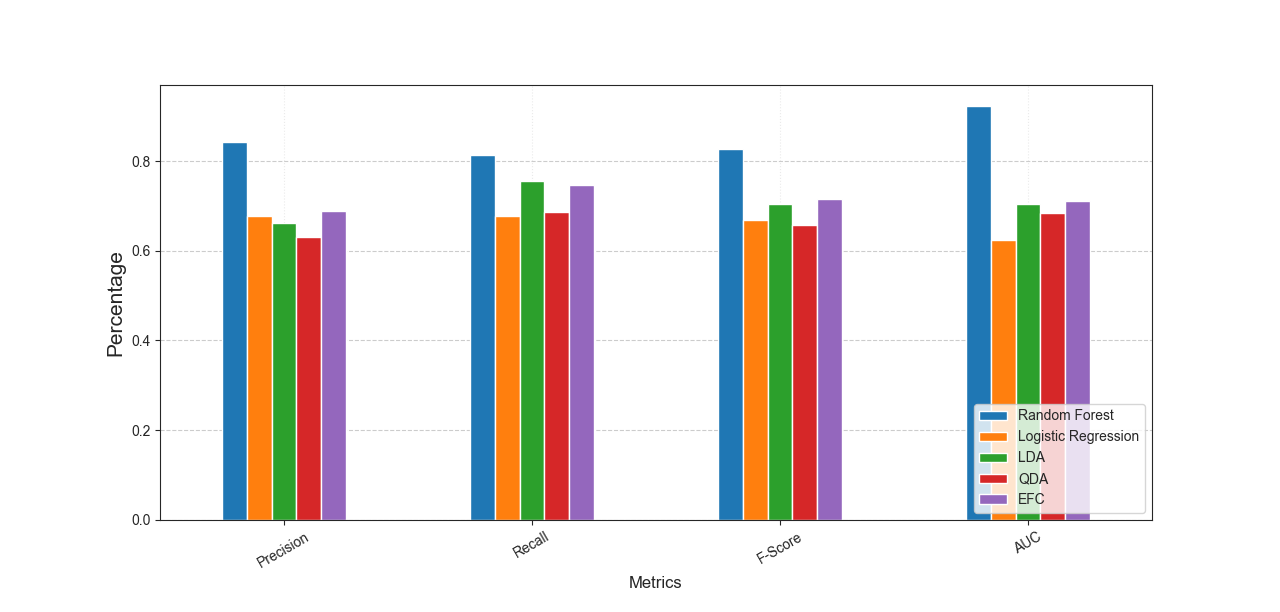
\includegraphics[width=0.85\textwidth]{image/barGraphMetrics.png} \\[\abovecaptionskip]
    
  \caption{The comparison of machine learning algorithms}\label{fig:metrics}
\end{figure*}


\subsection{Comparison of two detection Strategy}\label{sec:comparison}

{\bf \mas.} Considering the \cds (4,076 apps), the \fhc present
a total of {$1,395$} repackaged apps flagged as malware ({$34.22$\%} of the total number of repackaged apps), for which the repackaged app version calls at least one additional sensitive API. They explore accuracy metrics (such as Precision, Recall, and F-measure ($F_1$)), taking advantage of \vt to label the \cds and building a ground truth. Table~\ref{tab:accuracy} summarize the result of their study (First row). The study indicate that the \mas achieves an accuracy of 0.54 when considering the \cds. Nonetheless, the \mas fails to correctly classify $1,720$ assets as malware on the \cds (FN column, first row of Table~\ref{tab:accuracy}), and wrongly labeled the repackaged version of $220$ apps as malware (FP column). Therefore, the study reveals a {\bf lower performance} related to the accuracy of the approach, indicating that when considering the \cds, the accuracy of the \mas using DroidBot as test generate tool is just over $50$\%.

{\bf Flow Analysis.} Surprisingly, also considering the \cds (\apps pairs), we explored Flow Analysis with machine learning algorithm (Random Forest). As described in Section~\ref{sec:learning}, we trained $70$\% of the samples and tested on $30$\% of samples different from the trained ones. Our \cds cover \apps pair with $2,969$ original apps and $2,918$ malicious apps, totaling $5,887$ balanced samples. Accordingly, we trained our model on $4,120$ samples ($70$\% of $5,887$), and applied the trained model to $1,767$ samples ($30$\% of $5,887$). The Flow Analysis labeled a total of $690$ apps as malware, failed to correctly label $124$ assets as malware, and wrongly labeled the repackaged versions of $175$ samples (second row of Table~\ref{tab:accuracy}). Our Flow Analysis had a better performance, when compared to \mas, with an accuracy rate of $82$\%. From these results, we can conclude that Flow Analysis could be a complementary technique to \mas, improving the identification of malicious code in Android apps. In the next section, we present the results of combining both techniques for suspicious app detection.

\begin{finding}
The experimental results demonstrate that Network Flow analysis, combined with a machine learning algorithm, outperforms the \mas, with \fone of $0.82$. This proves to be an effective strategy to support the \mas for malware identification.
\end{finding}


\begin{table*}[h]
  \caption{Accuracy of both strategy on \cds.}
\centering{
  \begin{tabular}{lrrrrrr} \hline
    Dataset & TP   & FP  & FN  & Precision & Recall & $F_1$ \\
    \hline
    
    %\mas + Traces  & \sds (102)   & 67   & 18  & 2   & 0.78      & 0.97   & 0.87  \\
    \fhc : \mas (4,076 pairs)    & 1,175  & 220 & 1,720 & 0.84       & 0.40   & 0.54  \\
    Flow Analysis (1767 samples)~\footnote{Using Random Forest as ML algorithm}    & 690   & 175   & 124   & 0.79      & 0.84   & 0.82  \\
    %\mas + Traces  & \cds (1203)   & 214  & 326 & 245 & 0.39      & 0.46   & 0.42  \\ 
    \mas and Flow Analysis (4,076 pairs)    & 2,712   & 334   & 183   & 0.89      & 0.93   & 0.91  \\
    \hline
  \end{tabular}
  }
  \label{tab:accuracy}
\end{table*}


\subsection{Combining both Strategy}\label{sec:strategy}

Finally, to confirm our hypothesis from Section~\ref{sec:comparison}, we investigated the benefits of combining both approaches (\mas and Flow Analysis). The combined execution of both techniques correctly classified $2,712$ repackaged apps as malware (TP) and significantly decreased the number of (FN) from $1,720$ to $183$. However, this execution increased the number of (FP) from $220$ to $334$. The combination of both techniques proved to be more effective than the vanilla \mas. In summary, the results reveal that the combination of both techniques achieves an accuracy rate of $91$\% (third row of Table~\ref{tab:accuracy}).

To understand the benefits of each method, we further analyze the contribution of them for the accuracy. We report the raise of True Positive (TP) and False Positive (FP) for each technique in Figure~\ref{fig:venn}. The figure reveal that different approaches present different contribution to the final detection result.

\begin{finding}
When combining both techniques, we improve the overall accuracy (\fone) of \mas at malware detection, from $0.54$ to $0.91$ at \cds.
\end{finding}

\begin{figure}[t!]
  \centering
  \begin{tabular}{@{}c@{}}
    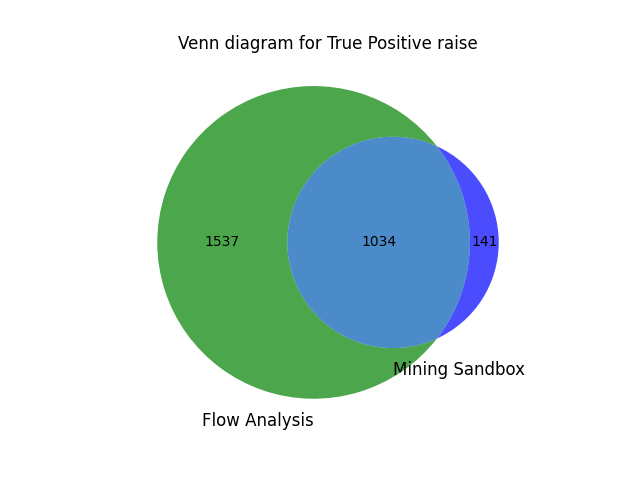
\includegraphics[width=0.54\textwidth]{image/vennTP.png} \\[\abovecaptionskip]
    \small (a) True Positive raise
  \end{tabular}

  \begin{tabular}{@{}c@{}}
    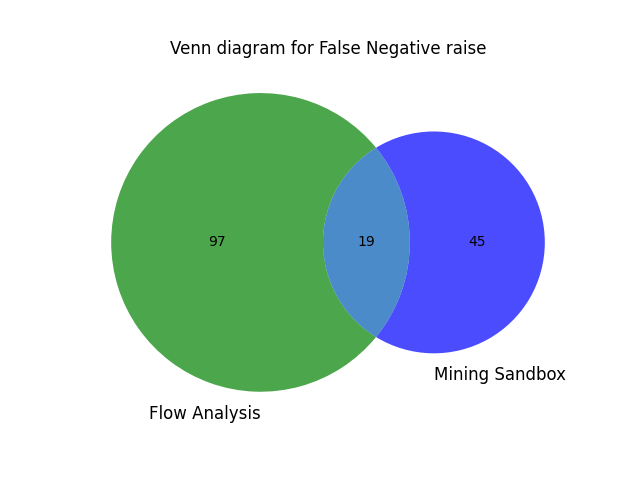
\includegraphics[width=0.54\textwidth]{image/vennFP.png} \\[\abovecaptionskip]
    \small (b) False Positive raise
  \end{tabular}

  \caption{Contribution to the final detection result}\label{fig:venn}
\end{figure}






\subsection{Detection Performance based on Malware Family}\label{sec:family}

In this section, we present the performance of our experiment based on each malware family. Since the number of samples in one family differs from the number in another, the overall detection rate is influenced more by the families with larger sample sizes. However, our results become inconsistent if we use the same number of samples for each family. To resolve the paradox, we present the results of the actual number of samples from the $10$ most representative families, which account for $87.83\%$ of all samples (Section~\ref{sec:familyDetection}). We also explored the detection rate of suspected recent malware samples. Although their families are unknown, we demonstrated that it is possible to improve the detection rate of suspicious apps by combining both strategies (Section~\ref{sec:unknowfamily}).


\subsubsection{Detection rate of 10 most representative malware families}\label{sec:familyDetection}

Among the $10$ most representative families, combining both strategies, the families with the highest earnings are \tjk and \gps. Regarding \tjk family malware, among the 34 samples evaluated, the \fhc flagged only 2 apps ($5.88$\%) as malicious. However, when combined with Flow Analysis, both approaches correctly labeled $32$ assets ($94.11$\%) as malicious, marking an $88.23$\% increase. Despite this, the \tjk family does not have as many representative samples as the \gps family, which accounts for $32.80$\% of all samples in the \cds, with $1,337$ samples. Among them, the \mas flagged $334$ samples ($12.93$\%) as malicious, while the combination of them indicated that $1,275$ ($95.36$\%) had suspicious activity, representing an $82.42$\% increase. Malware belonging to the \gps family automatically connects to networks, communicates with remote servers, and downloads and installs other apps or adware without the user’s knowledge\cite{DBLP:journals/jnca/WangCYYPJ19}. Due to their high network interaction, they are more easily detected by \net, proving it to be more efficient in detecting samples with malicious network behaviors.

Still, we should also note that $2$ families can correctly identified all samples as malware just with the \mas, \fm{airpush} and \fm{leadbolt}, with $120$ and $43$ samples respectively. At this case, the \net do not contribute to improving the ability to detect malicious activity, and just confirms the  maliciousness of the samples. The result reveals that the \mas remain effective for certain malware families. Figure~\ref{fig:bar} shows the detection performance of our strategies for the $10$ most representative families. In the figure, we can see that samples for the \gps family, had the the greatest benefit of the malware detection rate, with the support of flow analysis.



\begin{figure*}[h]
  \centering
  
    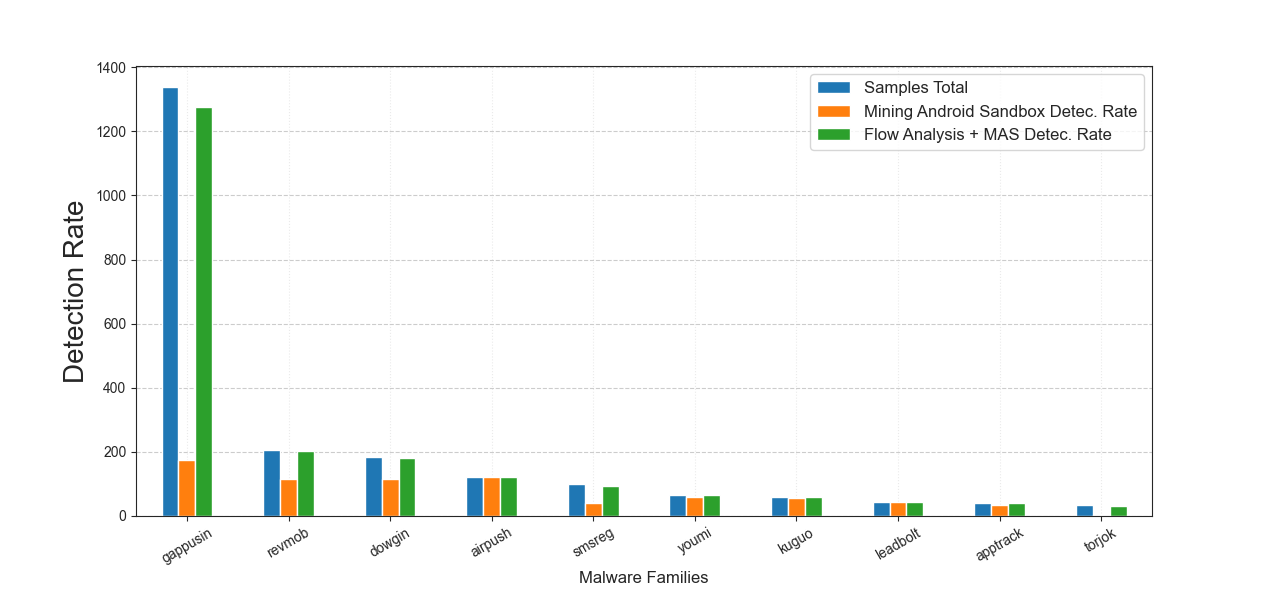
\includegraphics[width=\linewidth]{image/barGraph.png} \\[\abovecaptionskip]
    
  \caption{Detection Rate for Family}\label{fig:bar}
\end{figure*}

\begin{finding}

The combination of the \mas with \net, improve the malware detection rate for the \gps family (from $12.93$\% to $95.36$\%), the most representative family in \cds. This demonstrates the potential of this solution in detecting samples with malicious network behaviors.

\end{finding}


\subsubsection{Detection rate of unknown malware family}\label{sec:unknowfamily}

According to \vt, among the samples from our \cds, at least two \ses identified $253$ samples as malware. However, they were unable to specify their families. Since new malware emerges daily, accurately classifying recent malicious apps into their respective families is both challenging and time-consuming~\cite{DBLP:journals/compsec/WangTW21,DBLP:journals/compsec/ContiKP22}, which suggests that these are recent malware.

Although the specific families are unknown, the \mas detected suspicious activity in $114$ samples ($45.05$\%) from this set. On the other hand, when focusing solely on the results from the \net, for these unknown malware families, $124$ samples ($49.01$\%) were flagged as malicious. When we combine both approaches, the total number of apps flagged for suspicious activity increases to $170$ ($67.19$\%). Based on these results, we conclude that \net can effectively support the \mas, even for recently identified malicious apps, without malware family classification at the time of this research.

\begin{finding}

Even for recently malicious apps with unknown malware families, \net can support the \mas to improve the detection rate of apps with suspicious activities.

\end{finding}

\section{Discussion}\label{sec:discussion}
\section{Conclusions}\label{sec:conclusions}



In this paper, we propose a framework (\droidxpflow) for detecting Android malware using Network Traffic Analysis with ML support. As a first step, we created a dataset of network traffic (\fds) from the execution of $4,067$ repackaged apps, extracted from the dataset presented in the previous chapter. We then used our framework to investigate whether our method could overcome the limitations of the \mas, as discussed in the previous chapter, particularly for malware families that heavily interact with networks. Our evaluation demonstrates that \droidxpflow achieves a good performance in detecting Android malware, with an \fone of $0.89$. Although \droidxpflow builds upon the results of the state-of-the-art Mining Sandbox, we show that it is not a complete solution. Our evaluation reveals that there are samples in \fds that our framework fails to flag as malicious, whereas the \mas succeeds. We also highlight the limitations posed by our malicious samples quantity and discuss the importance of the number of samples used for training, as this can affect the accuracy of ML algorithms and, consequently, the effectiveness of our approach. As future work, we plan to collect, train, and analyze more malware samples to improve our malware detection solution by developing more sophisticated models. Additionally, we intend to explore more recent test generation tools that can better simulate user input, thereby making the collected traffic more closely resemble real-world scenarios.

\balance 

\bibliographystyle{IEEEtran}
\bibliography{ref}


\end{document}


